\documentclass[../main_proj3.tex]{subfiles}

\graphicspath{{\subfix{Figures/}}}

\begin{document}



\subsection{The Penning trap}

The Penning trap is used to confine charged particles using electromagnetic fields. The electric field  $\mathbf{E}$ is produced by the electrodes in the end-caps (components marked a) in the illustration and the ring (components marked b). The resulting electric field will trap the particle axially (z-plane) by some applied potential $V_0$,as will be shown by the derivation. To trap the particle radially (xy-plane) a magnetic field $\mathbf{B}$ with magnitude $B_0$ is set up by the magnet (component marked c) is used. By tuning the penning trap's field-strengths relative to the particle charge and mass ratio we can archive a trapped particle as illustrated by the red dot in the illustration.

\begin{figure}[h!]
    \centering
    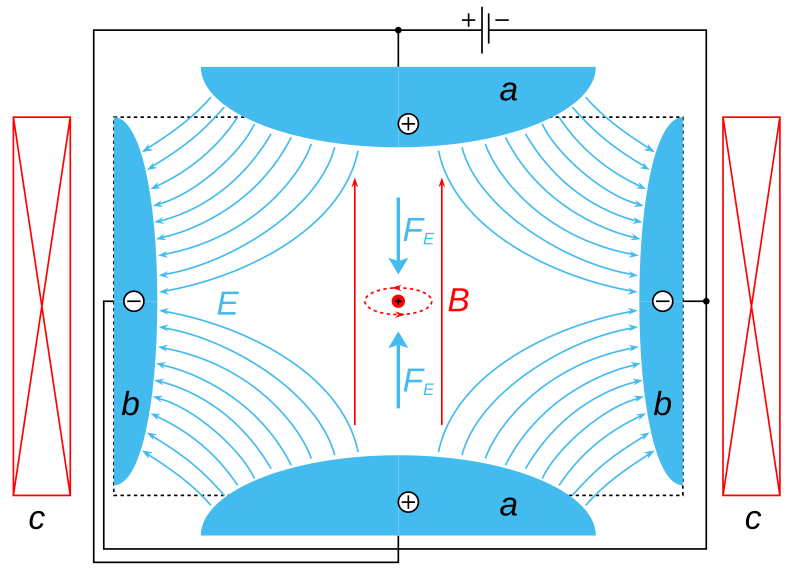
\includegraphics[width=0.9\linewidth]{Project 3/figures/Penning_Trap.png}
    \caption{The Penning trap key components include electrodes (a and b) and a magnet (c). Illustration from Wikipedia.org \cite{PenningTrapIllustration}.}
    \label{fig:Penning_trap}
\end{figure}


The electric field $\mathbf{E}$ is related to the electric potential $V$ by 
\begin{equation}
\label{eq:electric_field-electric_potential}
\mathbf{E} = - \nabla V \quad, 
\end{equation}

where we in this study consider an ideal Penning trap with the electric potential

\begin{equation}
\label{eq:electric_potential}
V(x,y,z) = \frac{V_0}{2d^{2}} (2z^{2} - x^{2} - y^{2}) \quad.
\end{equation}

The characteristic dimension $d=\sqrt{z_0^{2}+r_0^{2}/2}$ represents the length scale between electrodes defined by the distance from the center to the end caps $z_0$ and to the ring $r_0$. 

Solving equation \eqref{eq:electric_field-electric_potential} with $V$ from \eqref{eq:electric_potential} yields

\begin{equation}
\label{eq:solved_electric_field}
\begin{split}
\mathbf{E} & = - \nabla V \quad \\
& = - \frac{V_0}{2d^{2}} \nabla \left[2z^{2}-x^{2}-y^{2}\right] \\
& = \frac{V_0}{d^{2}} 
\bigl\langle 
x, y, -2z
\bigr\rangle \quad ,
\end{split}
\end{equation}

and the homogeneous magnetic field $\mathbf{B}$ is simply 
\begin{equation}
\label{eq:magnetic_field}
\mathbf{B} = \bigl\langle 
0, 0, B_0
\bigr\rangle \quad.
\end{equation}

 Modelling a charged particle as a point charge, it will set up an electric field in position $\mathbf{r}$ that is proportional to the particle charge $q$ and the distance from the particle and $\mathbf{r}$. If the Penning trap host's multiple point charges $\{q_1, \dots, q_n\}$ with positions $\{\mathbf{r}_1, \dots, \mathbf{r}_n\}$ they will set up an electric field in $\mathbf{r}$ given by the superposition of the individual fields, that is
\begin{equation}
\label{eq:electric_field_particles}
\mathbf{E} = k_e \sum\limits_{j=1}^n \frac{\mathbf{r}-\mathbf{r}_j}{|\mathbf{r}-\mathbf{r}_j|^{3}} \quad.
\end{equation}


\subsection{The equations of motion}

For the Penning trap the time evolution of a particle is given by Newton's second law 
\begin{equation}
\label{eq:newtons_second_law_Penning_trap}
m \mathbf{\ddot{r}}  = \sum_i \mathbf{F_i} \quad ,
\end{equation}
where $\mathbf{\ddot{r}}:=\frac{d^{2}\mathbf{r}}{dt^{2}}$ is the acceleration of the particle given its position in space $\mathbf{r}$. Further, the sum of forces $\sum_i \mathbf{F_i}$ on a particle is the Lorentz force

\begin{equation}
    \label{eq:Lorentz-force}
    \mathbf{F} = q\mathbf{E} + q \mathbf{v} \times \mathbf{B} \quad .
\end{equation}

Here $\mathbf{E}$ is given by equations \eqref{eq:solved_electric_field} and \eqref{eq:electric_field_particles} however, for this derivation we assume the number of particles to be one so we leave out the interactions. The cross product is solved as 

\begin{equation}
\label{eq:cross_product}
\begin{split}
q \mathbf{v} \times \mathbf{B} & =  q \bigl\langle 
\dot{x}, \dot{y}, \dot{z}
\bigr\rangle \times \bigl\langle 
0, 0, B_0
\bigr\rangle \\
&= qB_0 \bigl\langle
\dot{y}, -\dot{x}, 0
\bigr\rangle 
\end{split} \quad .
\end{equation}

Substituting equation \eqref{eq:solved_electric_field} \eqref{eq:cross_product} and \eqref{eq:Lorentz-force} into equation \eqref{eq:newtons_second_law_Penning_trap} yields the equation 

\begin{equation*}
m \mathbf{\ddot{r}} = q \frac{V_0}{d^{2}} 
\bigl\langle 
x, y, -2z
\bigr\rangle + qB_0 \bigl\langle
\dot{y}, -\dot{x}, 0
\bigr\rangle  \quad,
\end{equation*}

which for $\hat{e}_x$ becomes

\begin{equation}
\label{eq:eq_of_motion_x}
\begin{split}
m \ddot{x} & = \frac{2qV_0}{2d^{2}}x + qB_0 \dot{y}) \\
\ddot{x}  &= \omega_0 \dot{y} + \frac{1}{2} \omega_z^{2} x
\end{split}
\end{equation}

by defining $\omega_0 :=\frac{qB_0}{m}$ and $\omega_z^{2} := \frac{2qV_0}{md^{2}}$. Similarly for $\hat e_y$ the equation becomes 
\begin{equation}
\label{eq:eq_of_motion_y}
\ddot{y}  = \omega_0 \dot{x} + \frac{1}{2} \omega_z^{2} y \quad ,
\end{equation}

while for $\hat e_z$ we have $qB_0 \cdot 0$ so the expression simplifies to 

\begin{equation}
\label{eq:eq_of_motion_z}
\ddot z = - \omega_z^{2} z \quad .
\end{equation}

From these equations it is apparent that the magnetic field is only effecting the radial plane since $B_0$ is not present in equation \eqref{eq:eq_of_motion_z}. Since equation \eqref{eq:eq_of_motion_z} is a second order homogeneous differential equation the general solution is found by assuming $z(t)=e^{\lambda t}$ which yields the roots $\lambda= \pm i \omega_z^2$. Since these roots are only complex we get the general solution $z(t) = A\cos(\omega_z t) + B\sin(\omega_z t)$ \cite{NewcastleUniversity2024}.

The system of equations \eqref{eq:eq_of_motion_x}, \eqref{eq:eq_of_motion_y} and \eqref{eq:eq_of_motion_z} consists of three equations where equation \eqref{eq:eq_of_motion_x} and \eqref{eq:eq_of_motion_y} are coupled. To find a general solution, we start by rewriting these in terms of one differential equation by introducing a complex function $f(t)=x(t) + iy(t)$. Since $i= \sqrt{-1}$ is a \textit{const.} the first- and second-order derivatives become (using the dot notation and omitting the dependency towards $t$) $\dot f = \dot x + i \dot y$ and $\ddot f = \ddot x + i \ddot y$, respectively. By substituting equations \eqref{eq:eq_of_motion_x} and \eqref{eq:eq_of_motion_y}, solved for $x$ and $y$ respectively, into the complex function the pair can be compressed into one equation 

\begin{equation}
\label{eq:eq_of_motion_f}
\begin{split}
    f & = x + iy \\
    f & = (\ddot{x} - \omega_0 \dot{y}) \frac{2}{\omega_z^{2}} + i (\ddot{y} - \omega_0 \dot{x}) \frac{2}{\omega_z^{2}} \\
    \frac{1}{2} \omega_z^{2} f & = \ddot{x} + i\ddot{y} - \omega_0 \dot{y} - i \omega_0 \dot{x} \\
    \ddot{f} - \frac{1}{2} \omega_z^{2} f &= - \omega_0 ( \dot{y} +i \dot{x}) \\
    \ddot{f} & = \frac{1}{2} \omega_z^{2} f - i \omega_0 \dot{f}
\end{split}
\end{equation}

where we have identified that $\dot{y} +i \dot{x}$ in line four is equal to the imaginary unit times the complex conjugate of $f$; $i\dot{f}^* = i(\dot{x} - i\dot{y}) = \dot{y} + i \dot{x}$. Since $\dot{f}$ is a scalar and not a vector, it represents the \textit{speed} and not the \textit{velocity}, that consequence is that it is a real valued function of time and thus $\dot{f}^* = \dot{f}$. This equation describes the particle movement in the radial plane (xy-plane).

The general solution to \eqref{eq:eq_of_motion_f} is 
\begin{equation}
\label{eq:general_solution-eq_of_motion_f}
    f(t) = A_+ e^{-i(\omega_+ t + \phi_+)} + A_- e^{-i(\omega_- t + \phi_-)} \quad ,
\end{equation}

where $\phi_+$ and $\phi_-$ are constant phases, the amplitudes $A_+$ and $A_-$ are positive, and 
$$
\omega_\pm = \frac{\omega_0 \pm \sqrt{\omega_0^2 - 2\omega_z^2}}{2} \quad.
$$
For a given time $t$T he physical position of the particle is found by $x(t) = \text{Re}\big[f(t)\big]$ and $y(t) = \text{Im} \big[f(t)\big]$.

To obtain a bounded solution for the movement in the radial plane, we require $|f(t)| < \infty$ as $t\to \infty$. This implies that constraining the frequencies $\omega_\pm$ to be , as complex roots will make the exponent of the exponential in equation \eqref{eq:general_solution-eq_of_motion_f} positive, violating of the constraint in $f(t)$. To ensure real roots, we need 

\begin{equation}
\label{eq:frequency_constraint}
\begin{split}
    \omega_0^{2} - 2\omega_z^{2} &\geq 0 \\ 
    \frac{q^{2}B_0^{2}}{m^{2}} - 2\left(\frac{2qV_0}{md^{2}}\right) & \geq 0 \\
    \frac{q^{2}B_0^{2}}{m^{2}} & \geq 4 \frac{qV_0}{md^{2}} \\
    \frac{B_0^{2}d^{2}}{V_0} &\geq \frac{m}{q} \quad ,
\end{split}
\end{equation}

which means that the ratio between particle mass and charge must be less than or equal to the ratio between the squared product of the magnetic field strength and the characteristic length and the electric field strength. Physically, this implies that a stronger magnetic field is required if the electric field strength is increased. It also implies that increasing $B_0$ will make it easier to meet the stability requirement and that decreasing $d$ will reduce the stability given fixed values of $B_0$ and $V_0$.  



\subsection{Benchmark solution}

To benchmark the numerical modeling of this initial value problem, we will derive a specific analytical solution for a single particle $p$, defined in the project description \cite{prosjekttbeskrivelse3}. The particle $p$ has a charge $q$ and a mass $m$ while in the Penning trap. Initially, it occupies the position
$\mathbf{r_0} = \bigl\langle x(0), y(0), z(0) \bigr\rangle = \bigl\langle x_0, 0, z_0 \rangle$ and has the initial velocity $\mathbf{v}_0 = \bigl\langle 
\dot{x}(0), \dot{y}(0), \dot{z}(0)
\bigr\rangle = \bigl\langle 
0, v_0, 0 \bigr\rangle$. Further the specific solution to equation \eqref{eq:eq_of_motion_z} given the initial position $z_0$ is 
\begin{equation}
\label{eq:specific_solution-eq_of_motion_z}
z(t) = z_0 cos(\omega_z t) \quad.
\end{equation}

Further, the \textit{specific} solution to equation \eqref{eq:general_solution-eq_of_motion_f} is given by the amplitudes and phases 
\begin{equation*}
\begin{split}
    A_+ & = \frac{v_0 + \omega_-x_0}{\omega_- - \omega_+} \quad ,\\
    A_- & = - \frac{v_0 + \omega_+ x_0}{\omega_- - \omega_+} \quad , \\
    \phi_+ &= 0\quad , \\
    \phi_- & = 0    \quad.
\end{split}
\end{equation*}

We will use a singly-charge calcium ion (Ca$^{+}$) $p$ for this study with units; the micrometer ($\mathrm{\mu m}$) for length, microseconds ($\mathrm{\mu s}$) for time, the atomic mass unit ($\mathrm{u}$) for mass and the  elementary charge ($\mathrm{e}$) for charge.  This is done to reduce round-off errors that occur when working with very small numbers e.g. when considering the particle mass $m_{Ca^{+}} = 40.078 ~\mathrm{u}$ which is on the order of $10^{1}$ instead of $\mathcal{O}(m_{Ca} (kg)) = 10^{-26}$ (using $m_{Ca^{+}}\approx m_{Ca}$ since the mass of the added electron is negligible $\mathcal{O}(m_{e}(\text{kg}) = 10^{-31} << \mathcal{O}(m_{Ca})$).

In these units, the Coulomb constant is $k_e = 1.38935333 \times 10^5 \, \frac{\mathrm{u} \, (\mathrm{\mu m})^3}{(\mathrm{\mu s})^2 \, \mathrm{e}^2}$ and the derived SI units for the magnetic field strength (Tesla, $\mathrm{T}$) and the electric potential (Volt, $\mathrm{V}$) become $\mathrm{T} = 9.64852558 \times 10^1 \, \frac{\mathrm{u}}{(\mathrm{\mu s}) \, \mathrm{e}}$ and $\mathrm{V} = 9.64852558 \times 10^7 \, \frac{\mathrm{u} \, (\mathrm{\mu m})^2}{(\mathrm{\mu s})^2 \, \mathrm{e}}$.

Further, for a benchmark solution we set the magnetic field strength to $B_0 = 1.00\,\mathrm{T} \simeq 9.65 \times 10^1 \, \frac{\mathrm{u}}{(\mathrm{\mu s}) \, \mathrm{e}}$, the applied potential to $V_0 = 25.0\,\mathrm{mV} \simeq 2.41 \times 10^6 \, \frac{\mathrm{u} \, (\mathrm{\mu m})^2}{(\mathrm{\mu s})^2 \, \mathrm{e}}$ and the Penning trap characteristic dimension to $d = 500\,\mathrm{\mu m}$. Throughout the derived equations $V_0$ and $d$ only appear as the ratio $\frac{V_0}{d^{2}} = \frac{25 \mathrm{mV}}{500 \mathrm{\mu m}} = 9.65  \frac{\mathrm{u}}{(\mathrm{\mu s})^2 \, \mathrm{e}}$.


Taking into account the initial values $x_0 = z_0 = 20 \mathrm{\mu m}$ and $v_0 = 25 \mathrm{\mu m / \mu s}$ of the solution, simulating a single Ca$^{+}$ ion from $t=0\mathrm{\mu s}$ to $t= 50 \mathrm{\mu s}$ should be close to the position vector

\begin{equation*}
\begin{split}
\mathbf{r}(50)_{true} &= 
\left\langle
\begin{matrix}
\operatorname{Re}(f(50)), &\operatorname{Im}(f(50)),& z(50) 
\end{matrix} \right\rangle\\
&= \left\langle
\begin{matrix} 
21.7613,& 38.9772,& -19.8049 
\end{matrix}
\right \rangle \quad,
\end{split}
\end{equation*}
found by the specific analytical solution. 

\subsection{Multiple particles} 

Equations \eqref{eq:eq_of_motion_x}, \eqref{eq:eq_of_motion_y}, and \eqref{eq:eq_of_motion_z} yield elegant analytical solutions but do not allow for between-particle interactions. For a Penning trap with $n$ particles equation \eqref{eq:electric_field_particles} must be included in the Lorentz force calculations. For point charges $\{q_1, \dots, q_n\}$ with mass $\{m_1, \dots, m_n\}$ the set of equations become 
\begin{equation}
\label{eq:eq_of_motion_x_with_particleinteractions}
\ddot{x}_i - \omega_{0,i}\dot{y}_i - \frac{1}{2} \omega_{z,i}^2 x_i - k_e \frac{q_i}{m_i}\sum_{j\neq i}q_j \frac{x_i-x_j}{|\mathbf{r}_i - \mathbf{r}_j|^3} = 0 
\quad ,
\end{equation}
\begin{equation}
\label{eq:eq_of_motion_y_with_particleinteractions}
\ddot{y}_i + \omega_{0,i}\dot{x}_i - \frac{1}{2} \omega_{z,i}^2 y_i - k_e \frac{q_i}{m_i}\sum_{j\neq i}q_j \frac{y_i-y_j}{|\mathbf{r}_i - \mathbf{r}_j|^3} = 0
\quad ,
\end{equation}
and 
\begin{equation}
\label{eq:eq_of_motion_z_with_particleinteractions}
\ddot{z}_i + \omega_{z,i}^2z_i - k_e \frac{q_i}{m_i} \sum_{j\neq i}q_j \frac{z_i-z_j}{|\mathbf{r}_i - \mathbf{r}_j|^3} = 0 \quad. 
\end{equation}

Here the subscript $i$ denotes the particle of interest while $j$ denotes the other particles in the Penning trap. 

To solve this system of equations we will use numerical simulations from some initial values and propagate the solution forward in time using the forward Euler (FE) and the fourth order Runge-Kutta method (RK4) solving techniques. Both of these methods are made for first-order differential equations requring a re-formulation into a set of coupled first-order equations on the form $\dot{\mathbf{r}} = \mathbf{v}$ and $ \dot{\mathbf{v}} = \frac{\mathbf{F}}{m}$. Notation vise we now use  $\mathbf{v} = \langle\begin{matrix}v_x, &v_y, &v_z \end{matrix}\rangle:= \langle\begin{matrix}\frac{dx}{dt},&\frac{dy}{dt}, &\frac{dz}{dt}\end{matrix}\rangle$ instead of $\langle\begin{matrix}\dot{x},&\dot y, & \dot z \end{matrix}\rangle$. Further we will keep the radial plane decomposed, and not introduce any complex functions as we did to derive the general solution of equation \eqref{eq:general_solution-eq_of_motion_f}. 

In the x-plane we have equation \eqref{eq:eq_of_motion_x} and \eqref{eq:eq_of_motion_x_with_particleinteractions}. For a single particle  the form is achieved by writing 
\begin{equation*}
\begin{split}
\frac{dv_x}{dt} -\omega_0 v_y - \frac{1}{2} \omega_z^{2} x &=  0 \\
\frac{dv_x}{dt} - \frac{1}{m} \left( 
qB_0 v_y + q \frac{V_0}{d^{2}} x
\right) & = 0 
\end{split}    
\end{equation*}
where the units within the paranthesis becomes (dropping $\mu$ prefixes)
\begin{itemize}
    \item $\left[q B_0 v_y\right] = \mathrm{e \cdot \frac{u}{s~e} \cdot \frac{m}{s} = u \frac{m}{s^{2}}} = \text{mass}\frac{\text{length}}{\text{time}^{2}}$
    \item $\left[q \frac{V_0}{d^{2}} x\right] = \mathrm{e \cdot \frac{u~m^{2}}{s^{2}~e~m^{2}} \cdot m = u \frac{m}{s^{2}} } = \text{mass}\frac{\text{length}}{\text{time}^{2}}$
\end{itemize}

which is the same as force $F$. Hence 
\begin{equation}
\frac{d v_x}{dt} = \frac{1}{m} \left( 
qB_0 v_y + q \frac{V_0}{d^{2}} x
\right) = \frac {F_x}{m}\quad.
\end{equation}
With interactionsm, we again isolate $m_i^{-1}$ and the force expression for particle $i$ becomes 
\begin{equation*}
F_{x,i} = \left( 
q_iB_0 v_{y,i}  + q_i \frac{V_0}{d^{2}} x_i + k_e q_i \sum_{i\neq j} q_j \frac{x_i-x_j}{|\mathbf{r}_i - \mathbf{r}_j|^3} 
\right),
\end{equation*}
where the subscript $j$ refers to the remaining particles within the Penning trap. From the expressions for $F_x$ and $F_{x,i}$ we note that force will be the same for a single particle Penning trap weather or not the calculations are performed with one or the other since there are no $i\neq j$ for this trap. We therefor only focus on the expressions with interactions for the y- and z-plane

For equation \eqref{eq:eq_of_motion_y_with_particleinteractions} and \eqref{eq:eq_of_motion_z_with_particleinteractions} the expression for the force is 

\begin{equation*}
    F_{y,i} = \left( 
q_iB_0 v_{x,i}  + q_i \frac{V_0}{d^{2}} y_i + k_e q_i \sum_{i\neq j} q_j \frac{x_i-x_j}{|\mathbf{r}_i - \mathbf{r}_j|^3} 
\right), 
\end{equation*}
and 
\begin{equation*}
    F_{z,i} = \left(-2 \frac{q_iV_0}{d^{2}} + k_e q_i \sum\limits_{i\neq j} q_j \frac{z_i-z_j}{|\mathbf{r}_i - \mathbf{r}_j|^{3}}
    \right),
\end{equation*}
respectively. Using these expressions for the total force on a particle $i$ the vectors for the particle acceleration and speed is given by 
\begin{equation}
\label{eq:coupled_equations}
\begin{split}
    \langle\begin{matrix}
        \frac{dv_{x,i}}{dt}, & \frac{dv_{y,i}}{dt}, & \frac{dv_{z,i}}{dt}
    \end{matrix}\rangle &=
    \frac{1}{m_i}
    \langle\begin{matrix}
        F_{x,i}, & F_{y,i}, & F_{z,i}
    \end{matrix}\rangle , \\
    \langle\begin{matrix}
        \frac{dx_i}{dt}, & \frac{dy_i}{dt}, & \frac{dz_i}{dt}
    \end{matrix}\rangle &=
    \langle\begin{matrix}
        v_{x,i}, & v_{y,i}, & v_{z,i}
    \end{matrix}\rangle \quad.
\end{split}
\end{equation}


\subsection{Numerical simulations}

Considering a first order ODE 
$$\frac{dg}{dt} = f(t,g)\quad,$$ 
where $g(t)$ is unknown except for $g(t_0)$. For a simulation time $t_{sim}$ we have to set a resolution $n$ which dictates the number of steps we will divide the interval $[t_0, t_{sim}]$. This lets us define the step size
\begin{equation}
    \label{eq:step_size}
    h = \frac{t_{sim}-t_0}{n} \quad.
\end{equation}

To numerically simulate the time evolution of particle(s) in the Penning trap, we will now rewrite the derivative $\frac{dg}{dt}$ in terms of finite differences and solve for $g(t+h)$. However, the number of neighboring steps used for the estimation of $g(t+h)$ will be different between the methods.

\subsubsection{Forward Euler}

The Forward Euler (FE) method is derived by 
\begin{equation*}
    \begin{split}
        \frac{dg}{dt} &= f(t,g) \\
        \frac{g(t+h) - g(t)}{h} + \mathcal{O}(h) &= f(t,g) \\
        g(t+h) &\approx g(t) + hf(t,g) 
    \end{split}
\end{equation*}

where we have approximated by leaving out the $\mathcal{O}(h^{2})$ term. To discretize we define $g(t) \to g_l$ and $f(t, g)\to f_l$ so that we have the equation
\begin{equation}
\label{eq:next_timestep_forward_euler}
g_{l+1} = g_l+ h f_l = g_l + k \quad.
\end{equation}

For the coupled equations of \eqref{eq:coupled_equations} we let $f_l$ denote $F/m$ and use the Euler-Chromer method which yields the equations
\begin{equation}
\label{eq:coupled_equations_FE}
\begin{split}
    \left\langle\begin{matrix}
        v_{x,i,l+1} \\ v_{y,i,l+1}\\ v_{z,i,l+1}
    \end{matrix}\right\rangle &=
    \left\langle\begin{matrix}
        v_{x,i,l}+ hf_l\\ v_{y,i,l}+ hf_l\\ v_{z,i,l} + hf_l
    \end{matrix}\right\rangle, \\
    \left\langle\begin{matrix}
        x_{i,l+1} \\ y_{i,l+1}\\ z_{i,l+1}
    \end{matrix}\right\rangle &=
    \left\langle\begin{matrix}
        x_{i,l}+h v_{x,i,l+1}\\ y_{i,l} + h v_{y,i,l+1}\\ z_{i,l} + h v_{z,i,l+1}
    \end{matrix}\right\rangle \quad .
\end{split}    
\end{equation}

In the derivation of equation \eqref{eq:next_timestep_forward_euler} the Taylor series is truncated for all terms $k\geq 2$. The local error of the FE method is therefore $\mathcal{O}(h^{k}) = \mathcal{O}(h^{2})$ and the global error $\mathcal{O}(h^{k-1})=\mathcal{O}(h)$. This indicates that a smaller step size $h$ is needed to keep the error low when simulating with FE.

\subsubsection{Fourth order Runge-Kutta}

The fourth order Runge-Kutta method (RK4) corresponds to Taylor expanding $g_{i+1}$ four times. Considering the first order ODE from the FE derivation we can write the RK4 as
\begin{equation}
    \label{eq:next_timestep_RK4}
    \begin{split}
        k_1 &= hf(t_l, g_l) \\
        k_2 &= hf(t_l + \frac{1}{2}h, g_l +\frac{1}{2}k_1) \\
        k_3 &= hf(t_l + \frac{1}{2}h, g_l +\frac{1}{2}k_2) \\
        k_4 &= hf(t_l + h, g_l + k_3) \\
        g_{l+1} &= g_l + \frac{1}{6}(k_1 + 2k_2 + 2k_3 + k_4) \quad ,
    \end{split}
\end{equation}

where the weighting of the sum arises from Simpson's rule of numerical integration. Since RK4 is fourth order we truncate all terms $k\geq 5$ so the local error is of order $\mathcal{O}(h^{5})$ and hence the global error of order $\mathcal{O}(h^{4})$. Since our problem consists of the coupled set of equations in \eqref{eq:coupled_equations} and three spatial dimensions we use four vectors for position $\mathbf{k}_{\mathbf{r}, 1}, \dots, \mathbf{k}_{\mathbf{r}, 4}$ and four vectors for velocity $\mathbf{k}_{\mathbf{v}, 1}, \dots, \mathbf{k}_{\mathbf{v}, 4}$. Then after computing $\mathbf{k}_{\mathbf{r}, 1}$ and $\mathbf{k}_{\mathbf{v}, 1}$ for each particle, we temporarily evolve the system to $l+\frac{1}{2}h$, calculate $\mathbf{k}_{\mathbf{r}, 2}, \dots, \mathbf{k}_{\mathbf{v}, 2}$, etc. After the set of 8 vectors is calculated, we evolve the full system using equation \eqref{eq:next_timestep_RK4}. As in FE the function f(t, g) will be the calculation of the acceleration for the velocity vector and the velocity for the position vector.

\subsection{Experiments}

To enable investigations of the Penning trap physics we write a simulater enabled to solve equation \eqref{eq:coupled_equations} with either the FE or RK4 method.

\subsubsection{Testing the Penning trap}

To test the Penning trap functionality we will conduct a series of simulations. In addition to particle described under the benchmark solution we will have one more particle. Their initial values will be:
\begin{itemize}
    \item particle 1 (from benchmark solution)
    \begin{itemize}
        \item position: $\mathbf{r}= \langle 20, 0, 20 \rangle \mathrm{\mu m}$
        \item velocity: $\mathbf{v}= \langle 0, 25, 0 \rangle \mathrm{\mu m / \mu s}$
    \end{itemize}
    \item particle 2
    \begin{itemize}
        \item position: $\mathbf{r}= \langle 25, 25, 0 \rangle \mathrm{\mu m}$
        \item velocity: $\mathbf{v}= \langle 0, 40, 5 \rangle \mathrm{\mu m / \mu s}$.
    \end{itemize}
\end{itemize}

Firstly, to ensure a proper configuration of the Penning trap we will run a simulation with only particle 1 for a total time of $50 \mathrm{\mu s}$. We repeat the simulations for both FE and RK4 over a gradually higher amount of time steps $n_{\text{steps}} = \{4000, 8000, 16000, 32000\}$. From this we can calculate the relative error for the positions $\frac{|r-r_{\text{benchmark}}|}{r_{\text{benchmark}}}$ as well as the error convergence rate (see \cite{prosjekttbeskrivelse3} for details). Next we simulate two particles in the Penning trap with and without Coulomb forces to ensure that the particle interaction is working.

\subsubsection{Looking for resonance frequencies}

The uncover resonance frequencies in the Penning trap we will subject the particles to a time-dependent electromagnetic field and observe what fraction the Penning trap is able to contain over a simulation time of $500 \mathrm{\mu s}$. We perform the perturbations of $\mathbf{E}$ by varying the applied potential on the electrodes with $$
V_0(t) = V_0(1+fcos(\omega_vt))\quad. 
$$
Note that here we let $V_0$ denote the previously introduce constant magnitude and $V_0(t)$ denote the time-varying potential. Further, in this equation $f$ represents some constant amplitude which we will vary over the set $\{0.1,0.4,0.7\}$ and $\omega_v$ represents the angular frequency which we will vary over the set $\omega_{v, \text{broad set}} = \{0.2, 0.22, \dots, 2.48, 2.50\}$. To make the sample size larger the Penning trap will be imitated with 100 particles with randomly generated position and velocity vectors sampled from a normal distribution scaled by the characteristic length $d$.

Since simulations are computationally expensive we will perform the broad search over $\omega_{v, \text{broad set}}$ without interacting particles, i.e. their stability is decided by the Penning trap configuration. However we will further briefly investigate the effect of the Coloumb interactions on the stability by searching over one of the detected resonance domains with a finer meshed set for $\omega_v$.

\subsection{Tools}

All simulation code is written in cpp using mainly the armadillo library for vector hadnling. The exception is the specific solution for one particle that is written in Python with numpy. For plotting matplotlib and seaborn is used in jupyter notebooks. 

I have used the copilot codeium (\href{https://codeium.com/}{https://codeium.com/}) to aid with cpp syntax and python plotting. However I have not used it to develop any parts of the code unsupervised, all code structure is therefor created by me or taken from suggested structures from the project formulation.

\end{document}